
%(BEGIN_QUESTION)
% Copyright 2015, Tony R. Kuphaldt, released under the Creative Commons Attribution License (v 1.0)
% This means you may do almost anything with this work of mine, so long as you give me proper credit

\noindent
{\bf Capstone Assessment} (end of quarter)

\vskip 10pt

This performance assessment tests your mastery of many important instrumentation concepts.  You are to automate a pre-built process based on prototype diagrams you sketch of all instrument connections, and demonstrate the automatic control of this process.  All this must be done individually with no assistance from anyone else, within one lab session (not to exceed three hours).  You may refer to manufacturer documentation and/or textbooks, but not to personal notes, while building your loop. 

\vskip 10pt

{\bf You are entirely responsible for figuring out how the process works and what you must do to control it}, based on your inspection of it after it has been selected for you.  This includes identifying the process variable, the final control element, any loads, instrument model numbers, and locating manufacturer's documentation for the instrumentation.

\vskip 10pt

You may perform the assessment activity at any time in the quarter.  Successful completion counts as the ``mastery'' portion of the course exam(s).  If you do not pass, the instructor will work with you to correct the problem(s).  There is no grade penalty for repeated attempts, however successful completion is required to pass the course.

\vskip 10pt

In addition to exhibiting a steady-state control in automatic mode (i.e. the process variable follows changes made to the setpoint and settles at or near the setpoint value without oscillation after some time), the process must also meet the following criteria based on courses you have completed:

\begin{itemize}
\item{} If you have passed the {\it INST241} course, your transmitter and controller must be properly configured to register the process variable (in engineering units, not percent) over a range specified by the instructor.  Note: if the transmitter is analog rather than ``smart,'' the instructor will have you determine its ``As-Found'' range and direct you to range the loop controller to match the transmitter rather than calibrate the analog transmitter to a specified range.
\vskip 5pt
\item{} If you have passed the {\it INST252} course, the controller must be tuned for robust response to perturbations (changes) in either setpoint or load as selected by the instructor at or near a setpoint value also specified by the instructor.  ``Robust'' control is defined here as the controller compensating for perturbations as quickly as possible without creating any process variable oscillations (i.e. a {\it critically damped} response).  It will be your decision to use P, I, D, or any combination thereof in the controller's tuning.
\vskip 5pt
\item{} If you have passed the {\it INST260} course, you must connect a data acquisition unit (DAQ) to record a variable in the process selected by the instructor and display a trend graph on a personal computer networked to the DAQ.
\end{itemize}

\vskip 10pt

Given the time constraint of this assessment, you will not be required to cut and fit flexible conduit to the field instruments.  All other wiring must be neatly installed so as to avoid creating safety hazards (tripping, etc.) and confusion for other students assembling their loops.

Limited availability of components and physical space in the lab means that only a few students will be able to work on this assessment at once, so plan on attempting this {\it well before} the final due date!











\vfil \eject

\noindent
\centerline{{\bf Capstone project check-list (listed in sequential order)} \hskip 50pt Name: \underbar{\hskip 80pt}}

\vskip 10pt

Remember that you must work \underbar{independently} once the instructor assigns you a vest to wear.  Any consultation with classmates, use of personal notes, or deviation from your approved diagram(s) will result in immediate disqualification, which means you must take everything apart and re-try the capstone project on a different process.  Any damage done to the process or instrumentation will similarly result in disqualification, and you must repair the damage prior to re-trying the capstone project.  You are allowed to use manufacturer documentation, as well as any documentation provided by the instructor (e.g. textbooks).

\vskip 20pt

\centerline{\bf No teamwork is allowed while wearing the vest!}

\vskip 10pt

% No blank lines allowed between lines of an \halign structure!
% I use comments (%) instead, so that TeX doesn't choke.

$$\vbox{\offinterlineskip
\halign{\strut
\vrule \quad\hfil # \ \hfil & 
\vrule \quad\hfil # \ \hfil \vrule \cr
\noalign{\hrule}
%
% First row
{\bf Selection} & {\bf (Instructor writes/checks)} \cr
%
\noalign{\hrule}
%
% Another row
Instructor assigns a vest for you to wear &  \cr
%
\noalign{\hrule}
%
% Another row
Instructor selects a process for you to automate &  \cr
%
\noalign{\hrule}
%
% Another row
Instructor selects process variable range ({\it INST241 only}) &  \cr
%
\noalign{\hrule}
%
% Another row
Instructor selects setpoint/load \& SP value ({\it INST252 only}) & @ SP =  \cr
%
\noalign{\hrule}
%
% Another row
Instructor selects DAQ variable to measure ({\it INST260 only}) &  \cr
%
\noalign{\hrule}
%
% Another row
Instructor selects controller -- {\bf label with your name!} &  \cr
%
\noalign{\hrule}
%
% Another row
Instructor verifies no wiring connected to the process &  \cr
%
\noalign{\hrule}
} % End of \halign 
}$$ % End of \vbox

\vskip 10pt

\centerline{\bf The time clock starts now! \hskip 50pt Start time: \underbar{\hskip 80pt}}

\vskip 10pt

% No blank lines allowed between lines of an \halign structure!
% I use comments (%) instead, so that TeX doesn't choke.

$$\vbox{\offinterlineskip
\halign{\strut
\vrule \quad\hfil # \ \hfil & 
\vrule \quad\hfil # \ \hfil \vrule \cr
\noalign{\hrule}
%
% First row
{\bf Criterion} & {\bf (Instructor verifies)} \cr
%
\noalign{\hrule}
%
% Another row
You sketch basic loop diagram -- instructor verifies correctness &  \cr
%
\noalign{\hrule}
%
% Another row
You sketch DAQ connection diagram -- instructor verifies correctness &  \cr
%
\noalign{\hrule}
} % End of \halign 
}$$ % End of \vbox

\vskip 10pt

\centerline{\bf Now you may begin wiring and configuring the components}

\vskip 10pt

% No blank lines allowed between lines of an \halign structure!
% I use comments (%) instead, so that TeX doesn't choke.

$$\vbox{\offinterlineskip
\halign{\strut
\vrule \quad\hfil # \ \hfil & 
\vrule \quad\hfil # \ \hfil \vrule \cr
\noalign{\hrule}
%
% First row
{\bf Criterion} & {\bf (Instructor verifies)} \cr
%
\noalign{\hrule}
%
% Another row
Steady-state control in automatic mode &  \cr
%
\noalign{\hrule}
%
% Another row
Controller correctly registers the process variable ({\it INST241 only}) &  \cr
%
\noalign{\hrule}
%
% Another row
Controller responds robustly to perturbations ({\it INST252 only}) &  \cr
%
\noalign{\hrule}
%
% Another row
DAQ trend recording appears on a personal computer ({\it INST260 only}) &  \cr
%
\noalign{\hrule}
} % End of \halign 
}$$ % End of \vbox

\vskip 10pt

\centerline{\bf The time clock stops now! \hskip 50pt Stop time: \underbar{\hskip 80pt}}


% No blank lines allowed between lines of an \halign structure!
% I use comments (%) instead, so that TeX doesn't choke.

$$\vbox{\offinterlineskip
\halign{\strut
\vrule \quad\hfil # \ \hfil & 
\vrule \quad\hfil # \ \hfil \vrule \cr
\noalign{\hrule}
%
% First row
{\bf Criterion} & {\bf (Instructor verifies)} \cr
%
\noalign{\hrule}
%
% Another row
Instructor verifies all signal wires/tubes disconnected &  \cr
%
\noalign{\hrule}
%
% Another row
Instructor verifies controller reset to original configuration &  \cr
%
\noalign{\hrule}
%
% Another row
Instructor verifies DAQ is returned to team tool locker &  \cr
%
\noalign{\hrule}
%
% Another row
Instructor collects your diagrams &  \cr
%
\noalign{\hrule}
} % End of \halign 
}$$ % End of \vbox

\vskip 10pt

\centerline{\bf Your mastery score will not be recorded until \underbar{all} steps are complete!}







\vfil \eject

\centerline{\bf Notes on instrument ranging}

\vskip 10pt

An important criterion for the capstone project is that the loop instruments be properly ranged.  For students who have completed the INST241 course, this means both the transmitter and controller must be set to a specified measurement range, with the controller indicating the process variable in real ``engineering units'' (e.g. PSI or degrees F rather than just percent).

\vskip 10pt

The reason this is an issue at all is because loop controllers operating on 4-20 mA analog signals don't ``know'' what those signals are supposed to represent unless someone configures the controller with the proper range reflecting real-world conditions.  For example, if a student is assigned a temperature transmitter with a range of 300 to 800 degrees Fahrenheit, not only does the transmitter have to output 4 mA when sensing 300 $^{o}$F and output 20 mA when sensing 800 $^{o}$F, but the controller must display an indication of 300 $^{o}$F when it receives a 4 mA signal from the transmitter, and display an indication of 800 $^{o}$F when it receives a 20 mA signal from the transmitter.  None of this happens on its own -- the student must range the transmitter for 300-800 $^{o}$F input (and 4-20 mA output) as well as range the controller to display 300-800 $^{o}$F over its 4-20 mA input scale.  A typical loop is shown here with all instrument ranges displayed:

$$\includegraphics[width=15.5cm]{i00998x01.eps}$$

Analog (non-``smart'') transmitters, I/P transducers, and valve positioners are ranged using ``zero'' and ``span'' adjustments, typically screws or nuts.  The ranging of analog instruments is discussed in the ``Instrument Calibration'' chapter of the {\it Lessons In Industrial Instrumentation} textbook.

\vskip 10pt

Digital (``smart'') transmitters and valve positioners are ranged by setting LRV and URV parameters using a ``communicator'' device or a personal computer equipped with the appropriate interface and software.  This too is discussed in the ``Instrument Calibration'' chapter of the {\it Lessons In Industrial Instrumentation} textbook. 

\vskip 10pt

\filbreak

Digital electronic loop controllers similarly provide means to set the range values for interpreting any 4-20 mA signal input to them.  Exactly what these parameters are called and how they are accessed varies from one model and brand of loop controller to another.  Here are some examples:

\begin{itemize}
\item{} Siemens/Moore 352 controller: process variable range parameters are located in the ``Operator's Display'' function block (FB15):
\begin{itemize}

\item{} URV = {\it Process Hi}
\vskip 10pt
\item{} Siemens/Moore 352P and 353 controller: process variable range parameters are located in the ``Analog Input'' function block (AIN):
\begin{itemize}

\item{} URV = {\it Maxscale}
\vskip 10pt
\item{} Emerson DeltaV DCS: process variable range parameters are located in the ``Analog Input'' function block (AI) and ``PID'' function block (PID), both conforming to the FOUNDATION Fieldbus standard.  This standard for function block configuration is adhered to in the DeltaV system even if the loop in question uses analog (4-20 mA) signals.  Detailed information may be found in any FOUNDATION Fieldbus function block reference manual:
\begin{itemize}

\item{} (PID block) = the {\it PV\_SCALE} parameter contains both high and low range limits, engineering units (e.g. deg F), and decimal point position.
\vskip 10pt
\item{} Honeywell UDC 2500 controller: process variable input \#1 range parameters are located in the ``Input 1'' set-up group of parameters:
\begin{itemize}

\item{} URV = {\it IN1 HI}
\vskip 10pt
\item{} Automation Direct ``SOLO'' controller: process variable range parameters are located in the following registers:
\begin{itemize}

\item{} URV = {\it P3-3 Input Range High}
\vskip 10pt
\item{} Allen-Bradley PLC5, SLC500, and MicroLogix controllers: process variable scaling parameters are typically located either in a ``Scale'' instruction (SCL) or a ``Scale with Parameters'' instruction (SCP).  In either case, the instruction takes the raw count value from the input channel's analog-to-digital converter and scales it into the desired process variable display range.  A YouTube video on our BTCInstrumentation channel shows how to do this for the networked MicroLogix PLCs in the lab using the SCP instruction.  {\it Note: SCP instruction parameters may be edited online.  For this reason, downloading edits is not necessary for the MicroLogix PLCs in our lab.  In fact, it is very important that you \underbar{not} save or download the PLC program, because doing so may alter the PLC's network address and lead to communication problems.  Just make the changes while the PLC is in ``Run'' mode and then exit the program}:
\begin{itemize}

\item{} (SCP instruction LRV) = {\it Scaled Min.}
\item{} (SCP instruction URV) = {\it Scaled Max.}
\vskip 10pt
\item{} Allen-Bradley Logix5000 controller: process variable scaling parameters are located in the ``PID'' instruction (PID):
\begin{itemize}

\item{} URV = {\it .MAXS}
\end{itemize}
\end{itemize}








\vfil \eject

\centerline{\bf Notes on controller action}

\vskip 10pt

Another important criterion for the capstone project is that the loop controller execute the proper direction and magnitude of action in order to stabilize the process variable at setpoint.  For every student completing the capstone, this means setting the direction correctly (direct vs. reverse action) appropriate for the needs of the process, and configuring the tuning parameters (P, I, and D) to hold the process variable steady in automatic mode.  For students who have completed or are currently taking the INST252 course, this means tuning the controller for robust response to either setpoint or load perturbations (i.e. bringing the PV back to SP as quickly as possible without oscillation following sudden changes in either setpoint or load).

\vskip 10pt

If the controller happens to be programmed using function blocks, these important parameters will be found in the ``PID'' function block.  For other controller models, there will be a menu option with action (direct/reverse) and tuning (P/I/D) parameters.  Note that some controllers provide a quick-access feature to edit the PID tuning parameters, but generally not for changing the direction of action.  Here are some examples:

\vskip 10pt

\item{} Siemens/Moore 352 controller: control action parameters are located in the ``PID'' function block (FB13).  Note that the P, I, and D tuning parameters may be quickly accessed by pressing the ``Tune'' button rather than by entering the PID function block edit menu:
\begin{itemize}

\item{} Proportional (P) = {\it SPG1} as a unitless gain value
\item{} Integral (I) = {\it STI1} in units of minutes per repeat
\item{} Derivative (D) = {\it STD1} in units of minutes
\vskip 10pt
\item{} Siemens/Moore 352P and 353 controller: control action parameters are located in the ``PID'' function block (PID).  Note that the P, I, and D tuning parameters may be quickly accessed by pressing the ``Tune'' button rather than by entering the PID function block edit menu:
\begin{itemize}

\item{} Proportional (P) = {\it PG} as a unitless gain value
\item{} Integral (I) = {\it TI} in units of minutes per repeat
\item{} Derivative (D) = {\it TD} in units of minutes
\vskip 10pt
\item{} Emerson DeltaV DCS: control action parameters are located in the ``PID'' function block (PID) conforming to the FOUNDATION Fieldbus standard:
\begin{itemize}

\item{} Proportional (P) = {\it GAIN} as a unitless gain value
\item{} Integral (I) = {\it RESET} in units of seconds per repeat
\item{} Derivative (D) = {\it RATE} in units of seconds
\vskip 10pt
%\item{} Honeywell UDC 2500 controller: process variable input \#1 range parameters are located in the ``Input 1'' set-up group of parameters:
%\item{} LRV = {\it IN1 LO}
%\item{} URV = {\it IN1 HI}
%\vskip 10pt
%\item{} Automation Direct ``SOLO'' controller: process variable range parameters are located in the following registers:
%\item{} LRV = {\it P3-4 Input Range Low}
%\item{} URV = {\it P3-3 Input Range High}
%\vskip 10pt
\item{} Allen-Bradley PLC5, SLC500, and MicroLogix controllers: control action parameters are located in the ``PID'' instruction.  A YouTube video on our BTCInstrumentation channel shows how to do this for the networked MicroLogix PLCs in the lab:
\begin{itemize}

\item{} Proportional (P) = {\it Controller Gain} $K_c$ as a unitless gain value
\item{} Integral (I) = {\it Reset} $T_i$ in units of minutes per repeat
\item{} Derivative (D) = {\it Rate} $T_d$ in units of minutes
\vskip 10pt
\filbreak
\item{} Allen-Bradley Logix5000 controller: control action parameters are located in the ``PID'' instruction (PID):
\begin{itemize}

\item{} Proportional (P) = $K_p$ or $K_c$ as a unitless gain value
\item{} Integral (I) = $K_i$ in units of seconds per repeat
\item{} Derivative (D) = $K_d$ in units of minutes
\end{itemize}
\end{itemize}

\underbar{file i00998}
%(END_QUESTION)





%(BEGIN_ANSWER)

The only ``answer'' to this question is a properly documented and functioning instrument loop!
 
%(END_ANSWER)





%(BEGIN_NOTES)


%INDEX% Capstone assessment: end-of-quarter demonstration of automatically controlled process

%(END_NOTES)


